\documentclass[11pt]{article}

\newcommand{\yourname}{}

\def\comments{0}

%format and packages

%\usepackage{algorithm, algorithmic}

\usepackage{epsfig, graphicx}
\usepackage[noend]{algpseudocode}
\usepackage{amsmath, amssymb, amsthm}
\usepackage{enumerate}
\usepackage{enumitem}
\usepackage{framed}
\usepackage{verbatim}
\usepackage[margin=1.1in]{geometry}
\usepackage{microtype}
\usepackage{kpfonts}
\usepackage{palatino}
	\DeclareMathAlphabet{\mathtt}{OT1}{cmtt}{m}{n}
	\SetMathAlphabet{\mathtt}{bold}{OT1}{cmtt}{bx}{n}
	\DeclareMathAlphabet{\mathsf}{OT1}{cmss}{m}{n}
	\SetMathAlphabet{\mathsf}{bold}{OT1}{cmss}{bx}{n}
	\renewcommand*\ttdefault{cmtt}
	\renewcommand*\sfdefault{cmss}
	\renewcommand{\baselinestretch}{1.05}
\usepackage[usenames,dvipsnames]{xcolor}
\definecolor{DarkGreen}{rgb}{0.15,0.5,0.15}
\definecolor{DarkRed}{rgb}{0.6,0.2,0.2}
\definecolor{DarkBlue}{rgb}{0.2,0.2,0.6}
\definecolor{DarkPurple}{rgb}{0.4,0.2,0.4}
\usepackage[pdftex]{hyperref}
\hypersetup{
	linktocpage=true,
	colorlinks=true,				% false: boxed links; true: colored links
	linkcolor=DarkBlue,		% color of internal links
	citecolor=DarkBlue,	% color of links to bibliography
	urlcolor=DarkBlue,		% color of external links
}

\usepackage[boxruled,vlined,nofillcomment]{algorithm2e}
	\SetKwProg{Fn}{Function}{\string:}{}
	\SetKwFor{While}{While}{}{}
	\SetKwFor{For}{For}{}{}
	\SetKwIF{If}{ElseIf}{Else}{If}{:}{ElseIf}{Else}{:}
	\SetKw{Return}{Return}
	

%enclosure macros
\newcommand{\paren}[1]{\ensuremath{\left( {#1} \right)}}
\newcommand{\bracket}[1]{\ensuremath{\left\{ {#1} \right\}}}
\renewcommand{\sb}[1]{\ensuremath{\left[ {#1} \right\]}}
\newcommand{\ab}[1]{\ensuremath{\left\langle {#1} \right\rangle}}

%probability macros
\newcommand{\ex}[2]{{\ifx&#1& \mathbb{E} \else \underset{#1}{\mathbb{E}} \fi \left[#2\right]}}
\newcommand{\pr}[2]{{\ifx&#1& \mathbb{P} \else \underset{#1}{\mathbb{P}} \fi \left[#2\right]}}
\newcommand{\var}[2]{{\ifx&#1& \mathrm{Var} \else \underset{#1}{\mathrm{Var}} \fi \left[#2\right]}}

%useful CS macros
\newcommand{\poly}{\mathrm{poly}}
\newcommand{\polylog}{\mathrm{polylog}}
\newcommand{\zo}{\{0,1\}}
\newcommand{\pmo}{\{\pm1\}}
\newcommand{\getsr}{\gets_{\mbox{\tiny R}}}
\newcommand{\card}[1]{\left| #1 \right|}
\newcommand{\set}[1]{\left\{#1\right\}}
\newcommand{\negl}{\mathrm{negl}}
\newcommand{\eps}{\varepsilon}
\DeclareMathOperator*{\argmin}{arg\,min}
\DeclareMathOperator*{\argmax}{arg\,max}
\newcommand{\eqand}{\qquad \textrm{and} \qquad}
\newcommand{\ind}[1]{\mathbb{I}\{#1\}}
\newcommand{\sslash}{\ensuremath{\mathbin{/\mkern-3mu/}}}

%info theory macros
\newcommand{\SD}{\mathit{SD}}
\newcommand{\sd}[2]{\SD\left( #1 , #2 \right)}
\newcommand{\KL}{\mathit{KL}}
\newcommand{\kl}[2]{\KL\left(#1 \| #2 \right)}
\newcommand{\CS}{\ensuremath{\chi^2}}
\newcommand{\cs}[2]{\CS\left(#1 \| #2 \right)}
\newcommand{\MI}{\mathit{I}}
\newcommand{\mi}[2]{\MI\left(~#1~;~#2~\right)}

%mathbb
\newcommand{\N}{\mathbb{N}}
\newcommand{\R}{\mathbb{R}}
\newcommand{\Z}{\mathbb{Z}}
%mathcal
\newcommand{\cA}{\mathcal{A}}
\newcommand{\cB}{\mathcal{B}}
\newcommand{\cC}{\mathcal{C}}
\newcommand{\cD}{\mathcal{D}}
\newcommand{\cE}{\mathcal{E}}
\newcommand{\cF}{\mathcal{F}}
\newcommand{\cL}{\mathcal{L}}
\newcommand{\cM}{\mathcal{M}}
\newcommand{\cO}{\mathcal{O}}
\newcommand{\cP}{\mathcal{P}}
\newcommand{\cQ}{\mathcal{Q}}
\newcommand{\cR}{\mathcal{R}}
\newcommand{\cS}{\mathcal{S}}
\newcommand{\cU}{\mathcal{U}}
\newcommand{\cV}{\mathcal{V}}
\newcommand{\cW}{\mathcal{W}}
\newcommand{\cX}{\mathcal{X}}
\newcommand{\cY}{\mathcal{Y}}
\newcommand{\cZ}{\mathcal{Z}}

\newcommand{\opt}{\mbox{\textsc{opt}}}

%theorem macros
\newtheorem{thm}{Theorem}
\newtheorem{lem}[thm]{Lemma}
\newtheorem{fact}[thm]{Fact}
\newtheorem{clm}[thm]{Claim}
\newtheorem{rem}[thm]{Remark}
\newtheorem{coro}[thm]{Corollary}
\newtheorem{prop}[thm]{Proposition}
\newtheorem{conj}[thm]{Conjecture}
	\theoremstyle{definition}
\newtheorem{defn}[thm]{Definition}

\theoremstyle{theorem}
\newtheorem{prob}{Problem}


\newcommand{\course}{CS 3000: Algorithms \& Data}
\newcommand{\semester}{Spring 2022}

\newcommand{\psnum}{3}

\definecolor{cit}{rgb}{0.05,0.2,0.45} 

\begin{document}
{\Large 
\begin{center} \course\ --- \semester\ \end{center}}
{\large
\vspace{10pt}
\noindent Assignment ~\psnum}

\bigskip
{\large
\noindent Name: \yourname \vspace{2pt}\\ 
}
\vspace{15pt}
\begin{itemize}

\item Make sure to put your name on the first page.  If you are using the \LaTeX~template we provided, then you can make sure it appears by filling in the \texttt{yourname} command.

\item Solutions must be typeset in \LaTeX.  If you need to draw any diagrams, you may draw them by hand as long as they are embedded in the PDF.  We recommend using the source file for this assignment to get started.

\item Please review the academic integrity guidelines for assignments in the syllabus.

\item Finding solutions to homework problems on the web, or by asking
  students not enrolled in the class is strictly forbidden.

\end{itemize}
\newpage

%%%%%%%%%%%%PROBLEM 1 
\begin{prob}(4 + 4 = 8 points) Interval Scheduling Recap\end{prob}
This problem will test your understanding of dynamic programming by
having you run through the algorithm for interval scheduling that we
saw in class.  Consider the following input for the interval
scheduling problem:
\begin{center}
	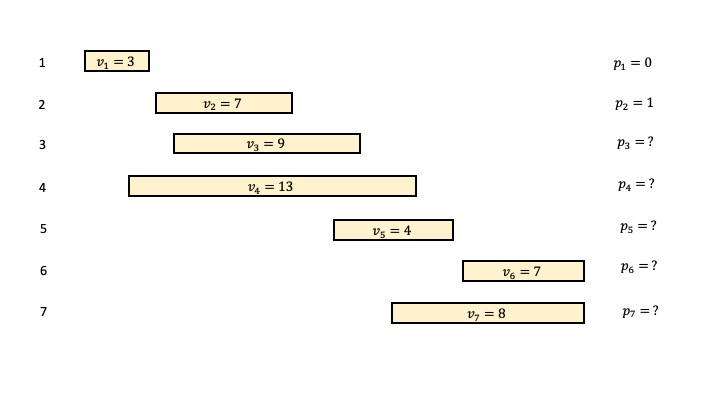
\includegraphics[width=\linewidth]{pics/p1.jpg}
\end{center}
\begin{itemize}
\item[{\bf (a)}] Recall that for any interval $i$, $p_i$ is the largest $j < i$ such that interval $j$ is compatible with $i$.  List the values for $p_i$ for $3 \le i \le 7$.

\begin{tabular}{ |c|c| } 
 \hline
 $i$ & $p(i)$ \\ 
 \hline
 3 & 1 \\ 
 4 & 0 \\ 
 5 & 2 \\ 
 6 & 4 \\ 
 7 & 3 \\ 
 \hline
\end{tabular}

\begin{algorithm}[H]
\Fn{$p(arr, i$)}{
  \For{$int j = i-1 \to 0$} {
    \If{$arr[j].end <= arr[i].start$} {
      \Return $j$
    }
  }
  \Return $0$
}
\end{algorithm}

  \item[{\bf (b)}] Fill out the dynamic programming table.  That is,
    for each value of $i = 0, 1, \ldots, 7$, determine both the value
    of $\opt(i)$ and whether or not the schedule $O_i$ includes
    schedule $i$.  Finally, write the optimal schedule $O_7$ and its
    value.
    
\begin{tabular}{ |c|c|c|c| } 
 \hline
 $i$ & OPT$(i)$ & $O_i$ & $contains$ $i?$ \\ 
 \hline
 0 & 0 & [0] & yes \\ 
 1 & 3 & [1] & yes \\ 
 2 & 10 & [1,2] & yes \\
 3 & 12 & [1,3] & yes \\
 4 & 13 & [4] & yes \\
 5 & 14 & [1,2,5] & yes \\
 6 & 21 & [1,2,5,6] & yes \\
 7 & 21 & [1,2,5,6] & no \\
 \hline
\end{tabular}

\end{itemize}

%%%%%%%%%%% PROBLEM 2
\begin{prob}
(10 + 10 + 5 = 25 points) Optimal location of stores
\end{prob}

You work for Chargepoint, a company that manufactures and installs electric vehicle charging stations. Chargepoint has just won a contract to install charging stations along I-90W starting in Boston. In order to maximize their usage you introduce a design constraint: no two chargers can be less than $f$ miles from each other. 

You have found out the location of a charger owned by rival EVGo is at a certain location on I-90W. There are no chargers west of this location, so your plan starts from this charger. You have identified exactly $n$ possible locations along I-90W for your chargers. The distances of each of these locations from the EVGo charger is provided in an array $d[1\ldots n]$ (in miles), where $d[i]$ is the distance of the $i^{th}$ location from the EVGo charger. The first possible location is $d[1]>0$ miles from the EVGo charger, and you are provided these distances such that $d[1]<d[2]<\ldots <d[n]$. Based on your CFO's analysis of potential usage and earnings, you have computed a value $v[i]$ for each location $i$. Given all of this data you would like to maximize the total value of the chargers to be installed, with the constraint that no two chargers are less than $f$ miles from each other. This constraint applies to the EVGo charger as well (i.e. the east-most charger you install cannot be less than $f$ miles west of the EVGo charger).

Your goal is to design a dynamic programming algorithm that takes
input the $d[1\ldots n]$ and $f$ and computes the locations where chargers will be installed.

\begin{itemize}
\item[{\bf (a)}] Let $\opt(i)$ denote the maximum value you can get
  for installing chargers in a subset of locations $1$ through $i$. Argue how the optimal substructure property holds for $\opt(i)$. Then give a recurrence to compute $\opt(i)$, and write the base case(s) for this recurrence.  Write a few sentences explaining why your recurrence is correct.

\item[{\bf (b)}] Using your recurrence, design a dynamic programming
  algorithm to produce the optimal set of charger locations to open.  You may use
  either a top-down or bottom-up approach.  Remember that your
  algorithm needs to produce the optimal set of charger locations, not only its
  value.  Your algorithm may output the set of locations as a list of its
  locations (in terms of distances from the EVGo charger along I-90W).

\begin{algorithm}[H]
$M \rightarrow []$ \\
$M[1] \rightarrow v[1]$ \\
\Fn{$findOPT(v, n)$} {
	\For{$i=2 \to n$} {
		$M[i] = max(M[i-1], v_i + M[p(i)])$\\
	}
	\Return M[n]
}

\Fn{$p(i)$} {
	\For{$j=i-1 \to 1$} {
		\If{$d[i] - d[j] <= f$} {
			\Return j
		}
	}
}

\Fn{$findChargers(d, v, i$)}{
	$S \rightarrow []$ \\
	\While{$i > 0$} {
		\If{$i == 1$} {
			$S.append(1)$ \\
			$i \rightarrow 0$
		}
		\ElseIf{$M[i] > v_i + M[p(i)]$} {
			$i -= 1$
		}
		\Else {
			$S.append(i)$\\
			$i \rightarrow p(i)$
		}
	}
	\Return S
}
\end{algorithm}

\item[{\bf (c)}]
  Analyze the running time and space usage of your algorithm.

\end{itemize}
(For full credit, the running time of your algorithm must be $O(n^2)$;
i.e., quadratic time or faster.  

%%%%%%%%%%% PROBLEM 3
\begin{prob}
(5 + 7 + 8 + 5 = 25 points) What's in a query?
\end{prob}

The space bar on Amit's smart phone is annoyingly small. Due to this when Amit types a query in Google, he often misses all the spaces. Thus the Google query shows up as a single word with no spaces and only lowercase text characters (e.g. ``whatisanalgorithm'' instead of ``what is an algorithm''). 

You are the engineer at Google working on the Google search query sanitation group. Your objective is to break such a query string into individual words. The query string may not even break into individual words that make sense (making this an illegitimate query)! To help with this, you have at your disposal a data structure that contains all permissible words, including all their forms (verbs, tenses, etc.). This data structure supports an O($1$)-time query $isWord(word)$ that answers true or false.

Devise a dynamic programming algorithm that will determine if a given single-word-without-space query can be broken down into a legitimate query, and if so, return the resulting multi-word string. 

\begin{itemize}
\item[{\bf (a)}] Write a recurrence relation to compute the answer. Argue how this answer contains within it solutions to smaller sub-problems. Briefly justify why your recurrence is correct.

\item[{\bf (b)}] Using your recurrence, design a dynamic programming algorithm to produce a ``Yes/No'' answer to whether the given query can be broken down into words.  You may use either a top-down or bottom-up approach.\\
\begin{algorithm}[H]
\Fn{$legitimateQuery(input$)}{
  boolean[] $map \rightarrow [False] * (input.length + 1)$ \\
  int[] $lastNeightbor \rightarrow [False] * (input.length + 1)$ \\
  $map[0] \rightarrow True$  \\ 

  \For{$i = 1 \to input.length$} {
    \For{$j = 0 \to i - 1$} {
      \If{$map[j]$ and $isWord(input[j, i])$} {
        $map[i] = True$ \\
        $lastNeightbor[i] = j$ \\
      }
    }
  }
  
  \If{$map[input.length]$} {
    \Return $''Yes''$
  }
  \Return $''No''$
}
\end{algorithm}
  
\item[{\bf (c)}] Extend your solution above so that if a query can be broken down into words, then the algorithm returns those words in order in a list. For example, ``whatisanalgorithm'' should return \[``what'',``is'',``an'',``algorithm''\]. If the query cannot be broken down into words, then your solution should return an empty list. \\
\begin{algorithm}[H]
\Fn{$legitimateQuery(input$)}{
  boolean[] $map \rightarrow [False] * (input.length + 1)$ \\
  int[] $lastNeightbor \rightarrow [False] * (input.length + 1)$ \\
  $map[0] \rightarrow True$  \\ 

  \For{$i = 1 \to input.length$} {
    \For{$j = 0 \to i - 1$} {
      \If{$map[j]$ and $isWord(input[j, i])$} {
        $map[i] = True$ \\
        $lastNeightbor[i] = j$ \\
      }
    }
  }
  
  \If{$map[input.length]$} {
    int $pointer = input.length$ \\
    string[] $output = []$ \\
    \While{$pointer != 1$} {
      $output.push(input[lastNeightbor[pointer], pointer])$ \\
      $pointer = lastNeightbor[pointer] $ \\
    }
    \Return $output$
  }
  \Return {[]}
}
\end{algorithm}

\item[{\bf (c)}]
  Analyze the running time and space usage of your algorithm in part (c).\\
\textbf{Space Analysis:} Space complexity for this algorithm is O(n) \\
\textbf{Time Analysis:} Time complexity is O(2n) \\

\end{itemize}

{\bf Extra credit (3+4 points):} In many cases it is possible to break down a query multiple ways: in this case your algorithm must favor a query with fewer words (i.e. longer strings). For example if the query is ``amendingconstitution'', it can be broken down into ``amending constitution'' or ``am ending constitution''. It should return the first.

Specify parts (a) and (b) for this problem (to return the breakdown of a query in the fewest number of words). 

%%%%%%%%%%% PROBLEM 4
\begin{prob}
(5 + 5 + 5 = 15 points) String shuffling (From Erickson)
\end{prob}

A {\em shuffle} of two strings $X$ and $Y$ is formed by interspersing the characters into a new string, keeping the characters of $X$ and $Y$ in the same order. For example the string {\color{red} BANANAANANAS} is a shuffle of the strings {\color{blue}BANANA} and {\color{red}ANANAS} in several different ways: 
\begin{itemize}
    \item{{\color{blue}BANANA}{\color{red}ANANAS}}
    \item{{\color{blue}BAN}{\color{red}ANA}{\color{blue}ANA}{\color{red}NAS}}
    \item{{\color{blue}B}{\color{red}AN}{\color{blue}AN}{\color{red}A}{\color{blue}A}{\color{red}NA}{\color{blue}NA}{\color{red}S}}
\end{itemize}

Similarly the strings {\color{red}PRODGYRNAMAMMIINCG} and {\color{red}{DYPRONGARMAMMICING} are both shuffles of {\color{blue}DYNAMIC}} and {\color{red}PROGRAMMING} in the following ways:

\begin{itemize}
    \item{{\color{red}PRO}{\color{blue}D}{\color{red}G}{\color{blue}Y}{\color{red}R}{\color{blue}NAM}{\color{red}{AMMI}}{\color{blue}I}{\color{red}N}{\color{blue}C}{\color{red}G}}
    \item{{\color{blue}DY}{\color{red}PRO}{\color{blue}N}{\color{red}G}{\color{blue}A}{\color{red}R}{\color{blue}M}{\color{red}AMM}{\color{blue}IC}{\color{red}ING}}
    \end{itemize}
    
Given three strings $X[1\ldots m]$, $Y[1\ldots n]$ and $Z[1\ldots m+n]$ design a solution based on dynamic programming to determine whether $Z$ is a shuffle of $X$ and $Y$.

\begin{itemize}
\item[{\bf (a)}] Write a recurrence relation to compute the answer. Argue how this answer contains within it solutions to smaller sub-problems. Briefly justify why your recurrence is correct.

\item[{\bf (b)}] Using your recurrence, design a bottom-up dynamic programming
  algorithm to produce a ``Yes/No'' answer to whether $Z$ is a shuffle of $X$ and $Y$. \\
  
\begin{algorithm}[H]
\Fn{$isStringShuffled(string1, string2, stringShuffled$)}{
 \If{stringShuffled.length != string1.length + string2.length} {
   \Return False \\
 }
  $boolean[string1.length + 1][string2.length + 1] map \rightarrow [][]$ \\
  
  \For{$i = 0 \to string1.length$} {
    \For{$j = 0 \to string2.length$} {
      \If{$i == 0$ and $j == 0$} {
        $map[i][j] = True$
      }
      \ElseIf{$i == 0$} {
        $map[i][j] = map[i][j-1]$ and $string2[j-1] == stringShuffled[i+j-1]$
      }
      \ElseIf{$j == 0$} {
        $map[i][j] = map[i-1][j]$ and $string1[i-1] == stringShuffled[i+j-1]$
      }
      \Else {
        $map[i][j] =(string1[i-1] == stringShuffled[i+j-1])$ and $(string2[j-1] == stringShuffled[i+j-1])$
      }
    }
  }
  
  \Return $map[string1.length][string2.length]$
}
\end{algorithm}
  
\item[{\bf (c)}]
  Analyze the running time and space usage of your algorithm.\\
\textbf{Space Analysis:} Space complexity for this algorithm is O(m*n) \\
\textbf{Time Analysis:} Time complexity is O(m*n) \\

\end{itemize}





\end{document}
